\uuid{P6Td}
\exo7id{5909}
\titre{exo7 5909}
\auteur{rouget}
\organisation{exo7}
\datecreate{2010-10-16}
\isIndication{false}
\isCorrection{true}
\chapitre{Analyse vectorielle}
\sousChapitre{Forme différentielle, champ de vecteurs, circulation}
\module{Géométrie}
\niveau{L2}
\difficulte{}

\contenu{
\texte{
(Un calcul de $\int_{0}^{+\infty} \frac{\sin x}{x}\;dx$).
}
\begin{enumerate}
    \item \question{$r$ et $R$ sont deux réels strictement positifs tels que $r<R$. On considère le contour $\Gamma$ orienté suivant

$$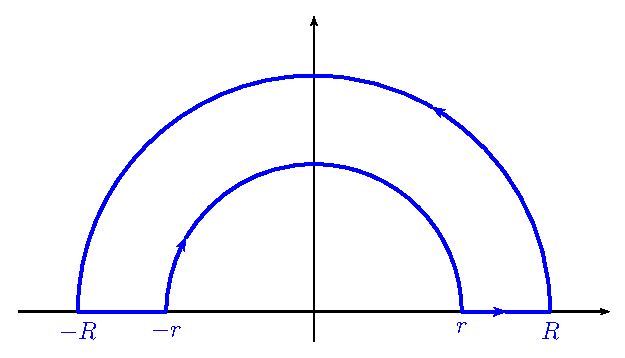
\includegraphics{../images/P6Td-1}$$



Calculer l'intégrale de la forme différentielle 

\begin{center}
$\omega= \frac{e^{-y}}{x^2+y^2}((x\sin x-y\cos x)dx+(x\cos x+y\sin x)dy)$
\end{center}

le long de ce contour orienté.}
\reponse{La forme différentielle $\omega$ est de classe $C^1$ sur $\Rr^2\setminus\{(0,0)\}$. D'après le théorème de \textsc{Schwarz}, sur tout ouvert étoilé $\Omega$ contenu dans $\Rr^2\setminus\{(0,0)\}$, la forme différentielle $\omega$ est exacte si et seulement si la forme différentielle $\omega$ est fermée.

Pour $(x,y)\in\Rr^2\setminus\{(0,0)\}$, posons $P(x,y)= \frac{e^{-y}}{x^2+y^2}(x\sin x-y\cos x)$ et $Q(x,y)= \frac{e^{-y}}{x^2+y^2}(x\cos x+y\sin x)$. Pour $(x,y)\in\Rr^2$,

\begin{align*}\ensuremath
 \frac{\partial Q}{\partial x}(x,y)&= \frac{-2xe^{-y}}{(x^2+y^2)^2}(x\cos x+y\sin x)+ \frac{e^{-y}}{x^2+y^2}(-x\sin x+\cos x+y\cos x)\\
 &= \frac{e^{-y}}{(x^2+y^2)^2}(-2x(x\cos x+y\sin x)+(x^2+y^2)(-x\sin x+\cos x+y\cos x))\\
 &= \frac{e^{-y}}{(x^2+y^2)^2}((-x^2+y^2+x^2y+y^3)\cos x+(-2xy-x^3-xy^2)\sin x),
\end{align*}

et

\begin{align*}\ensuremath
 \frac{\partial P}{\partial y}(x,y)&= \frac{-e^{-y}}{x^2+y^2}(x\sin x-y\cos x)+ \frac{-2ye^{-y}}{(x^2+y^2)^2}(x\sin x-y\cos x)+ \frac{e^{-y}}{x^2+y^2}(-\cos x)\\
 &= \frac{e^{-y}}{(x^2+y^2)^2}(-(x^2+y^2)(x\sin x-y\cos x)-2y(x\sin x-y\cos x)-(x^2+y^2)\cos x)\\
 &= \frac{e^{-y}}{(x^2+y^2)^2}((-x^2+y^2+x^2y+y^3)\cos x+(-2xy-x^3-xy^2)\sin x)\\
 &= \frac{\partial Q}{\partial x}(x,y).
\end{align*}

Finalement, la forme différentielle $\omega$ est exacte sur tout ouvert étoilé $\Omega$ contenu dans $\Rr^2\setminus\{(0,0)\}$.

On choisit $\Omega=\Rr^2\setminus\{(0,y),\;y\leqslant0\}$. $\Omega$ est un ouvert étoilé (en tout point de la forme $(0,y)$, $y>0$) de $\Rr^2$ contenant le contour fermé $\Gamma$. Puisque $\omega$ est exacte sur $\Omega$, on sait alors que $\int_{\Gamma}^{}\omega=0$.}
    \item \question{En déduire $\int_{r}^{R} \frac{\sin x}{x}\;dx$ en fonction d'une autre intégrale.}
\reponse{Le contour $\Gamma$ est constitué de $4$ arcs :

\textbullet~$\Gamma_1$ est l'arc $t\mapsto(t,0)$, $t$ variant en croissant de $r$ à $R$,

\textbullet~$\Gamma_2$ est l'arc $t\mapsto(R\cos t,R\sin t)$, $t$ variant en croissant de $0$ à $\pi$.

\textbullet~$\Gamma_3$ est l'arc $t\mapsto(t,0)$, $t$ variant en croissant de $-R$ à $-r$,

\textbullet~$\Gamma_4$ est l'arc $t\mapsto(r\cos t,r\sin t)$, $t$ variant en décroissant de $\pi$ à $0$.

D'après la question 1), $\int_{\Gamma_1}^{}\omega+\int_{\Gamma_2}^{}\omega+\int_{\Gamma_3}^{}\omega+\int_{\Gamma_4}^{}\omega=0$.

\begin{align*}\ensuremath
\int_{\Gamma_1}^{}\omega&=\int_{r}^{R}(P(x(t),y(t))x'(t)+Q(x(t),y(t))y'(t))\;dt=\int_{r}^{R}P(t,0)\;dt\\
 &=\int_{r}^{R} \frac{1}{t^2}\times t\sin t\;dt=\int_{r}^{R} \frac{\sin t}{t}\;dt.
\end{align*}

De même, $\int_{\Gamma_3}^{}\omega=\int_{-R}^{-r} \frac{\sin t}{t}\;dt=\int_{r}^{R} \frac{\sin t}{t}\;dt$ (puisque la fonction $x\mapsto \frac{\sin x}{x}$ est paire) et donc $\int_{\Gamma_1}^{}\omega+\int_{\Gamma_3}^{}\omega=2\int_{r}^{R} \frac{\sin x}{x}\;dx$ puis pour tout $(r,R)\in]0,+\infty[^2$ tel que $r<R$,

\begin{center}
$\int_{r}^{R} \frac{\sin x}{x}\;dx=- \frac{1}{2}\left(\int_{\Gamma_2}^{}\omega+\int_{\Gamma_4}^{}\omega\right)$.
\end{center}

Ensuite,

\begin{align*}\ensuremath
\int_{\Gamma_2}^{}\omega&=\int_{0}^{\pi}(P(R\cos t,R\sin t)(-\sin t)+Q(R\cos t,\sin t)(\cos t))\;dt\\
 &=\int_{0}^{\pi}e^{-R\sin t}((\cos t\sin(R\cos t)-\sin t\cos(R\cos t))(-\sin t)+(\cos t\cos(R\cos t)+\sin t\sin(R\cos t))(\cos t))\;dt\\
 &=\int_{0}^{\pi}e^{-R\sin t}\cos(R\cos t)\;dt.
\end{align*}

De même, $\int_{\Gamma_4}^{}\omega=\int_{\pi}^{0}e^{-r\sin t}\cos(r\cos t)\;dt=-\int_{0}^{\pi}e^{-r\sin t}\cos(r\cos t)\;dt$ et on a montré que

\begin{center}
\shadowbox{
$\forall(r,R)\in]0,+\infty[^2$, $r<R\Rightarrow\int_{r}^{R} \frac{\sin x}{x}\;dx= \frac{1}{2}\left(\int_{0}^{\pi}e^{-r\sin t}\cos(r\cos t)\;dt-\int_{0}^{\pi}e^{-R\sin t}\cos(R\cos t)\;dt\right)$.
}
\end{center}}
    \item \question{En faisant tendre $r$ vers $0$ et $R$ vers $+\infty$, déterminer la valeur de $\int_{0}^{+\infty} \frac{\sin x}{x}\;dx$.}
\reponse{\textbullet~Etudions $\lim_{R \rightarrow +\infty}\int_{0}^{\pi}e^{-R\sin t}\cos(R\cos t)\;dt$. Pour $R>0$,

\begin{align*}\ensuremath
\left|\int_{0}^{\pi}e^{-R\sin t}\cos(R\cos t)\;dt\right|&\leqslant\int_{0}^{\pi}e^{-R\sin t}\left|\cos(R\cos t)\right|\;dt\leqslant\int_{0}^{\pi}e^{-R\sin t}\;dt=2\int_{0}^{\pi/2}e^{-R\sin t}\;dt\\
 &\leqslant2\int_{0}^{\pi/2}e^{-R(2t/\pi)}\;dt\;(\text{la fonction sinus étant concave sur}\;\left[0, \frac{\pi}{2}\right])\\
 &= \frac{\pi}{R}\left[-e^{-2Rt/\pi}\right]_0^{\pi}= \frac{\pi}{R}(1-e^{-2R})\\
 &\leqslant \frac{\pi}{R}.
\end{align*}

Comme $ \frac{\pi}{R}$ tend vers $0$ quand $R$ tend vers $+\infty$, $\lim_{R \rightarrow +\infty}\int_{0}^{\pi}e^{-R\sin t}\cos(R\cos t)\;dt=0$. On en déduit que pour tout $r>0$, l'intégrale $\int_{r}^{+\infty} \frac{\sin x}{x}\;dx$ converge en $+\infty$ et que

\begin{center}
\shadowbox{
$\forall r>0$, $\int_{r}^{+\infty} \frac{\sin x}{x}\;dx= \frac{1}{2}\int_{0}^{\pi}e^{-r\sin t}\cos(r\cos t)\;dt$.
}
\end{center}

\textbullet~Etudions maintenant $\lim_{r \rightarrow 0}\int_{0}^{\pi}e^{-r\sin t}\cos(r\cos t)\;dt$. Soit $\begin{array}[t]{cccc}
F~:&[0,+\infty[\times[0,\pi]&\rightarrow&\Rr\\
 &(r,t)&\mapsto&e^{-r\sin t}\cos(r\cos t)
\end{array}$.

- Pour tout réel $r\in[0,+\infty[$, la fonction $t\mapsto F(r,t)$ est continue par morceaux sur $[0,\pi]$.

- Pour tout réel $t\in[0,\pi]$, la fonction $r\mapsto F(r,t)$ est continue sur $[0,+\infty[$.

- Pour tout $(r,t)\in[0,+\infty[\times[0,\pi]$, $|F(r,t)|\leqslant1=\varphi(t)$ où $\varphi$ est une fonction continue par morceaux et intégrable sur le segment $[0,\pi]$.

D'après le théorème de continuité des intégrales à paramètres, la fonction $r\mapsto\int_{0}^{\pi}e^{-r\sin t}\cos(r\cos t)\;dt$ est continue sur $[0,+\infty[$. On en déduit que

\begin{center}
$\lim_{r \rightarrow 0}\int_{0}^{\pi}e^{-r\sin t}\cos(r\cos t)\;dt=\int_{0}^{\pi}e^0\cos(0)\;dt=\pi$,
\end{center}

et finalement que

\begin{center}
\shadowbox{
$\int_{0}^{+\infty} \frac{\sin x}{x}\;dx= \frac{\pi}{2}$.
}
\end{center}}
\end{enumerate}
}
